\section{Structure of Hydrogen}
\subsection{Fine structure}
\subsubsection{Relativistic correction to kinetic energy}
The lowest-order correction Hamiltonian due to relativistic correction to kinetic energy is 
\begin{equation}\label{eqn:relativistic_hamiltonian}
    H'_r = -\df{p^4}{8m^3c^2}
\end{equation}
Exploiting the Hermiticity of $p$, the first-order correction is
\begin{equation}
    E_r^1=-\df{1}{8m^3c^2}\ang{p^2\psi|p^2\psi}
\end{equation}
For our unperturbed $|\psi\ra$, which are solved for non-relativistically, $p^2=2m(E-V)$, so 
\begin{equation}\begin{aligned}\label{eqn:rel_corr}
    E^1_r &= -\df1{2mc^2}\ang{(E-V)^2} \\ 
        &= -\df1{2mc^2}\left(E_n^2 - 2E_n \ang{V} + \ang{V^2}\right) \\ 
        &=-\df{(E_n)^2}{2mc^2}\left[\df{4n}{l+1/2}-3\right]
\end{aligned}\end{equation}
Several quantities which are handy in such evaluations when we use the basis $n, l, m_l$
\begin{equation}
    \ang{\df 1 r} = \df 1 {n^2 a} \quad \ang{\df 1 {r^2}} = \df 1 {(l+1/2)n^3a^2}\quad 
    \ang{\df 1 {r^3}} = \df 1 {l(l+1/2)(l+1)n^3a^3}
\end{equation}

The perturbation is spherically symmetric, so $L^2, L_z$ 
commute with both $H, H'_r$ and $|n, l, m\ra$ are distinct eigenstates of $(L^2, L_z)$, 
taken together, allowing us to use nondegenerate perturbation theory. 
Relativistic correction to the kinetic energy lifts the $l$-degeneracy. 
Our complete set of commuting observables (recall~\ref{def:csco}) are $H, L^2, L_z, S^2, S_z$. 

\subsubsection{Spin-orbit coupling}
From the electron's frame, the proton's motion generates a magnetic field which 
couples to the electron spin. 
\begin{equation}\label{eqn:spin_orbit_coupling}
    H'_{\mathrm{so}} = \left(\df{e^2}{8\pi \epsilon_0}\right)\df 1 {m^2c^2r^3}\bf{S\cdot L}
\end{equation}
The energy spectrum is degenerate in $m, m_s$ yet 
${[\mbf S\cdot \mbf L, L_z], [\mbf{S\cdot L}, S_z]}\neq 0$. 
Therefore we cannot use $m, s$ as 
our quantum numbers. Consider instead the total angular momentum 
\begin{equation}\label{def:J}
    \bf{J\equiv L + S}
\end{equation}
We propose an addition of angular momentum transformation, which 
replaces the complete set of commuting observables for a Hamiltonian 
from $L^2, L_z, S^2, S_z$ with $J^2, L^2, S^2, J_z$ corresponding to 
quantum numbers $j, l, s, m_j$. We first need to 
verify commutativity with $H'_{\mrm{so}}$. 
\begin{proposition}
    $[\mbf J, \mbf{S\cdot L}] = 0$

    \textit{Proof:} Without loss of generality consider $J_z$, 
    \[\begin{aligned} 
        [J_z, \mbf{S\cdot L}] 
            &= [S_z+L_z, S_xL_x+S_yL_y+S_zL_z] \\ 
            &= [S_z, S_x]L_x + [S_z, S_y]L_y + [L_z, L_x]S_x + [L_z, L_y]S_y \\ 
            &= S_yL_x - S_xL_y + L_yS_x - L_xS_y = 0
    \end{aligned}\]
\end{proposition}
Also note that $\mbf{S\cdot L} = \df 1 2 (J^2 - L^2 - S^2)$, 
so $H'_{\mrm{so}}$ commutes with $L^2, S^2, J^2, J_z$. 
\begin{proposition}
    $H'_{\mrm{so}}$ commutes with $J^2, L^2, S^2, J_z$. 

    \prf The previous proposition shows that $H'_{\mrm{so}}$ commutes with $J_z$. 
    To show commutativity with the other observables, note that 
    \[ 
        \mbf{S\cdot L} = \df 1 2 (J^2 - L^2 - S^2)
    \] 
    The three operators $L^2, S^2, J^2$ pairwise commute. 
\end{proposition}
The eigenvalues of $\mbf{L\cdot S}$ are then
\[ 
    \df{\hb^2}2\left[j(j+1)-l(l+1)-s(s+1)\right]
\]
Substituting total spin $s=1/2$ 
\begin{figure}[h!] % The [h!] tries to place the figure "here" as closely as possible
    \centering
    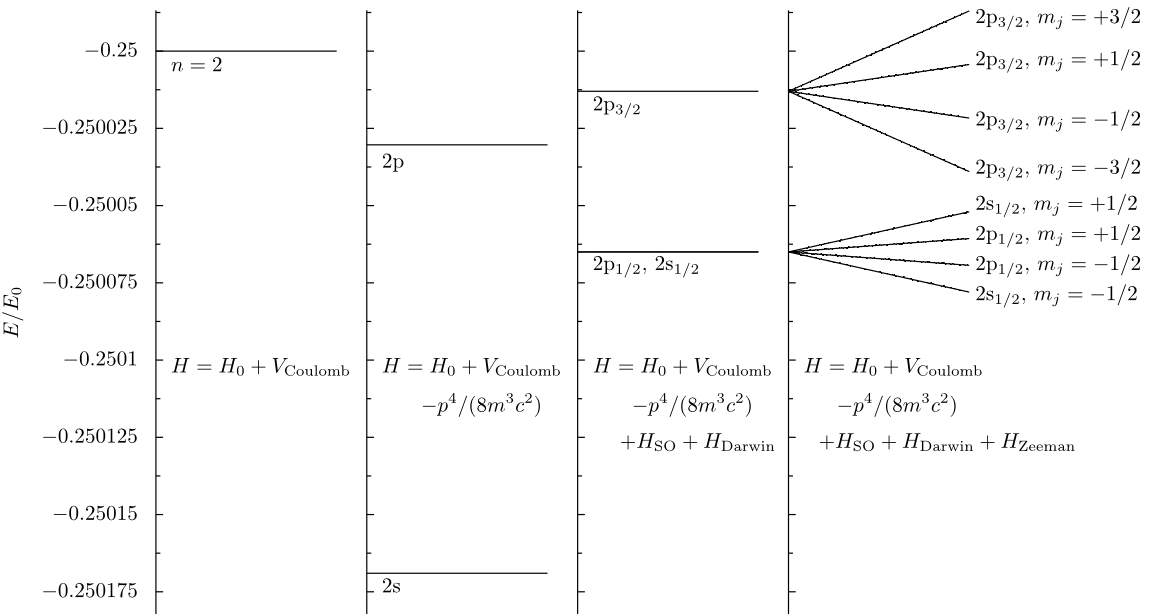
\includegraphics[width=1\linewidth]{src/n=2_hydrogen_fs.png}
    \caption{Fine-structure and Zeeman corrections for $n=2$}
    \label{fig:fs_zeeman}
\end{figure}
\begin{equation}
    E^1_{\mrm{so}}=\df{(E_n)^2}{mc^2}\cdot \df{n\left[j(j+1)-l(l+1)-3/4\right]}{l(l+1/2)(l+1)}
\end{equation}
Luckily, this combines neatly with the contribution from the 
relativistic correction to give the fine structure correction 
\begin{equation}
    E^1_{\mrm{fs}}=\df{(E_n)^2}{2mc^2}\left(3-\df{4n}{j+1/2}\right)
\end{equation}
\begin{table}[h!]
    \centering
    \begin{tabular}{|c|c|c|c|c|}
    \hline
    $n$ & $j$ & $l$ & $m_j$ & degeneracy \\ 
    \hline
    $1$ & $1/2$ & $\{0\}$ & $\{\pm 1/2\}$ & $2$ \\
    $2$ & $1/2$ & $\{0, 1\}$ & $\{\pm1/2\}$ & $4$ \\
        & $3/2$ & $\{1\}$    & $\{\pm1/2, \pm 3/2\}$ & $4$ \\
    $3$ & $1/2$ & $\{0\}$  & $\{\pm 1/2\}$ & $2$ \\
        & $3/2$ & $\{1, 2\}$ & $\{\pm 1/2, \pm3/2\}$ & $8$ \\
        & $5/2$ & $\{2\}$ & $\{\pm 1/2, \pm 3/2, \pm5/2\}$ & $6$ \\
    \hline
    \end{tabular}
    \caption{Energy levels of a spin $1/2$ particle for $n\leq 3$, arranged in $(n, j)$
    \label{tbl:hydrogen_fs}}
\end{table}
Combined with the Bohr formula, the energy now depend on both $n, j$. 
\begin{mdframed}
\begin{equation}\label{eqn:fs_energy_level}
    E_{nj} = -\df{(E_0)^2}{n^2}\left[1 + \df{\alpha^2}{n^2}\left(\df{n}{j+1/2} - \df 3 4\right)\right]
\end{equation}
\end{mdframed}
Our complete set of commuting observables are $H, L^2, S^2, J^2, J_z$ 
corresponding to quantum numbers $n, l, s, j, m_j$. 
Given $n$, we still have considerable degeneracy in $j, l, m_j$ (table~\ref{tbl:hydrogen_fs}).

\subsection{Zeeman effect}
Zeeman effect characterizes the energy corrections of an atom under external magnetic field. 
\begin{definition}[gyromagnetic ratio]
    The gyromagnetic ratio $\gamma$ of a system is the ratio between its magnetic moment and angular momentum. 
    \[ 
        \bm \mu = \gamma \mbf L
    \] 
    For a classically rotating body, $\gamma = \df q{2m}$. 
\end{definition}
\begin{definition}[Bohr magneton]
    The Bohr magneton provides the natural unit for gyromagnetic ratio of atomic systems. 
    \[ 
        \mu_B \equiv \df {e\hb}{2m_e}
    \] 
\end{definition}

For an electron, the gyromagnetic ratio for orbital motion and spin are different: that for the spin is roughly 
twice its classical value. Note that $\bm \mu$ scales inversely with mass. 
\begin{equation}
    \bm \mu = \bm \mu_l + \bm \mu_s = \df {\mu_B}{\hb}\left(\mbf L + 2\mbf S\right)
\end{equation}
In an external magnetic field $\mbf B$, a hydrogenic atom has the following correction 
\begin{equation}
    H'_Z = -\bm \mu \cdot \mbf B=\df {\mu_B} {\hb}\left(\mbf L + 2\mbf S\right)\cdot \mbf B
\end{equation}

\subsubsection{Weak-field Zeeman effect}

When $B\ll B_{\mrm{int}}$, we let $H^0=H_{\mrm{Bohr}}+H'_{fs}$. The zeroth-order eigenstates are given by 
by $L^2, S^2, J^2, J_z$. Without loss of generality, let $\mbf B = B\hat {\mbf z}$, then ($Z$ is for Zeeman)
\begin{equation}\label{eqn:zeeman_hamiltonian}
    H'_Z = \df{\mu_B B}{\hb}\left(L_z + 2S_z\right)
\end{equation}
After we have thus aligned the external field in the $z$-direction, 
the correction $H'_Z$ commutes with our complete set of 
operators and is diagonal in the $l, s, j, m_j$ basis, in which case 
\begin{equation}\begin{aligned}
    E^1_Z &= \df{\mu_B B}{\hb}\la L_z + 2S_z\ra \\ 
          &= \df{\mu_B B}{\hb}\left(J_z + \la S_z\right)\ra 
\end{aligned}\end{equation}
We now consider $\la S_z\ra$: the total angular momentum $\mbf J = \mbf L + \mbf S$ is constant, so the 
time average of $\mbf S$ is its projection along $\mbf J$ (see Griffiths for detailed explanation) 
\begin{equation}\begin{aligned}
    \la S_z\ra &= \df{\la \mbf{S\cdot J}\ra}{J^2}J_z \\ 
    &= \la \df 1 2\left(J^2 + S^2 - L^2\right)\ra\df{\hb m_j}{j(j+1)} \\
    &= \df{j(j+1)+s(s+1)-l(l+1)}{2j(j+1)}\hb m_j \\ 
    &= (g_J-1) m_j
\end{aligned}\end{equation}
Here we introduced the Landé $g$-factor $g_J$. The matrix element for energy correction is 
\begin{equation}
    \la n, l, s, j, m_j | H'_Z | n, l, s, j, m_j \ra = E^1_Z = \mu_B g_J m_j B
\end{equation}
Note that this correction is linear in $m_j$. 
Combined with equation~\ref{eqn:fs_energy_level}, the energy levels accounting for fine structure and 
weak-field Zeeman effect is 
\begin{equation}
    E_{nj} = -\df{(E_0)^2}{n^2}\left[1 + \df{\alpha^2}{n^2}\left(\df{n}{j+1/2} - \df 3 4\right)\right] + \mu_B g_Jm_j B
\end{equation}

\subsubsection{Strong-field Zeeman effect}
When the external magnetic field dominates the proton's magnetic field, we take $H^0=H_{\mrm{Bohr}}+H'_Z$ and 
$H'_{\mrm{fs}}$ to be the perturbation. 

Originally, $H_{\mrm{Bohr}}$ is degenerate in 
$l, s, m_l, m_s$, and equation~\ref{eqn:zeeman_hamiltonian} suggests that the 
states with the same $m_l+2m_s$ are degenerate eigenstates of $H^0$. 
To apply non-degenerate perturbation theory, 
our basis must arise from a set commuting operators complementing $H^0, H'_{\mrm{fs}}$ 
which additionally lifts the degeneracy in $l, s, m_l+2m_s$. 
One such set is $L^2, S^2, J^2, J_z$. 
\begin{equation}
    E^1_{\mrm{fs}} = \la n, l, m_l, m_s | H'_r + H'_{\mrm{so}} | n, l, m_l, m_s\ra 
\end{equation}
Here $\la H'_r\ra$ commutes with the operators for our basis, so we can use equation~\ref{eqn:rel_corr}. 
For the spin-orbit term, $\la S_zL_z\ra = \hb^2m_lm_s$. Substitute the indeterminate quotient 
with $1$ when $l=0$.
\begin{equation}
    E^1_{\mrm{fs}} = -\df{E_0}{n^3}\alpha^2 \left[\df 3 {4n} - \df{l(l+1) - m_lm_s}{l(l+1/2)(l+1)}\right]
\end{equation}

\begin{figure} % The [h!] tries to place the figure "here" as closely as possible
    \centering
    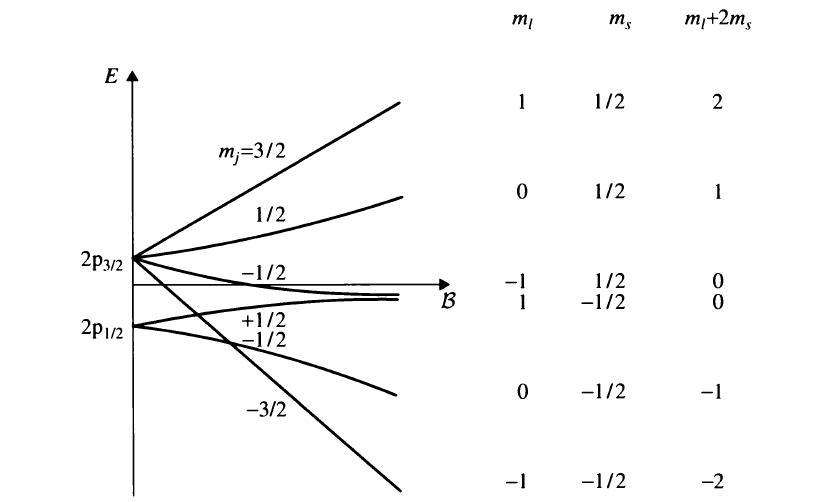
\includegraphics[width=1\linewidth]{src/zeeman.png}
    \caption{Zeeman effect for $n=2, l=1$}
    \label{fig:zeeman}
\end{figure}

Equation~\ref{eqn:zeeman_hamiltonian} dominates in the strong field regime,
while the fine structure characterized by~\ref{eqn:relativistic_hamiltonian}, 
\ref{eqn:spin_orbit_coupling} dominates in the weak field regime. 
The quantum numbers which distinguish between energy levels
in the strong-field regime is then $n, l, s, m_l+2m_s$, while those in the 
weak-field regime are $n, l, s, j, m_j$. The asymptotic slope in the figure above is 
determined by $m_l+2m_s$. 

\begin{figure}
    \centering
    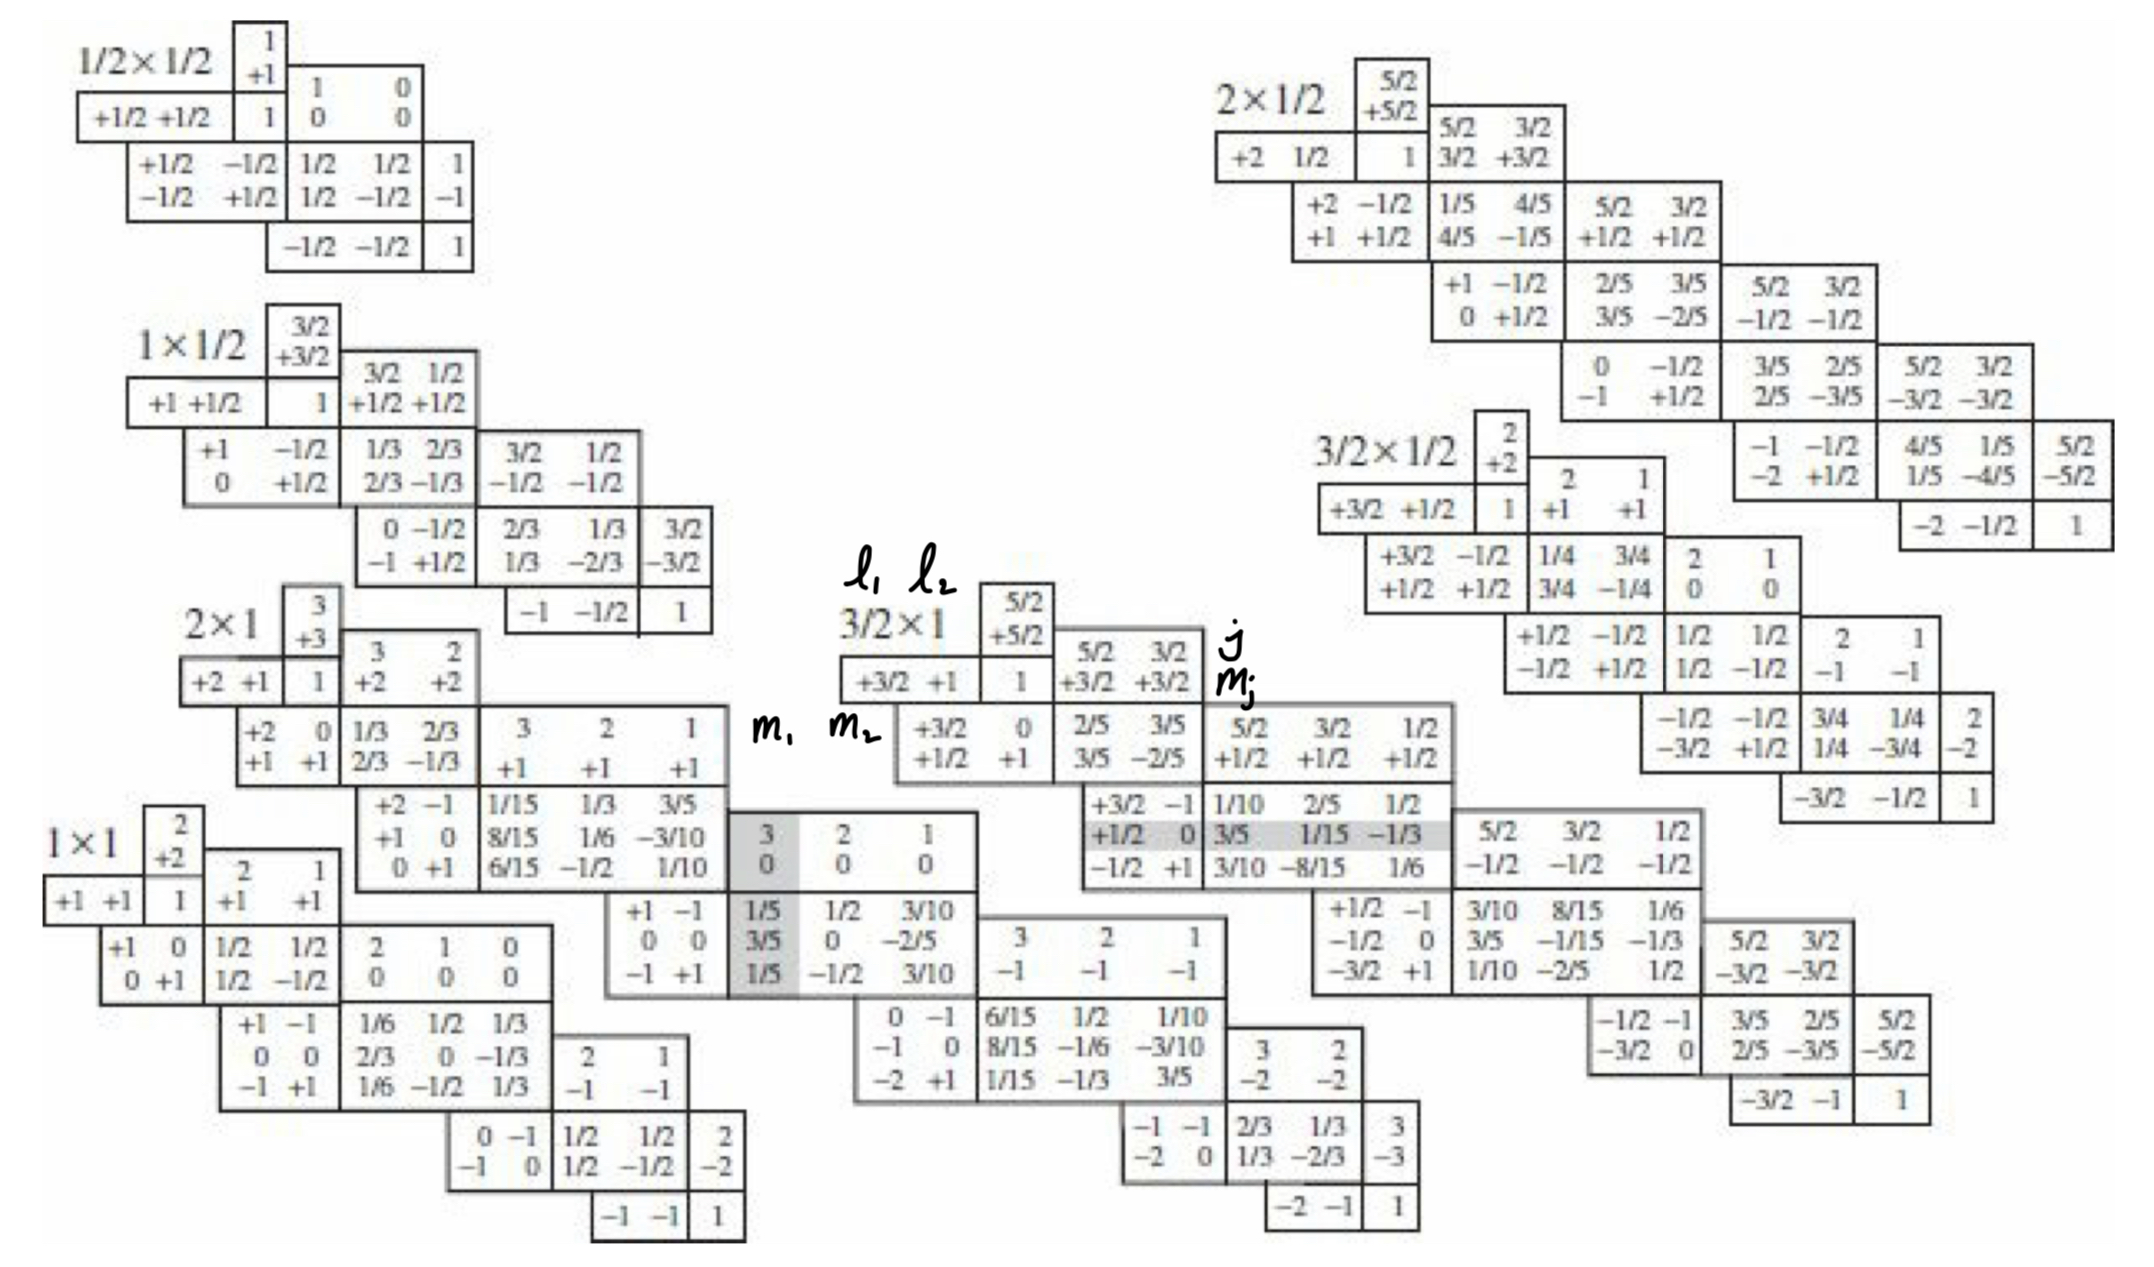
\includegraphics[width=1\linewidth]{src/clebsch-gordan.jpeg}
    \caption{Clebsch-Gordan coefficients}
    \label{fig:cg_coef}
\end{figure}

% \subsection{Hyperfine structure}
% The magnetic spin-dipole of a proton and electron are, for $g_p\approx 5.59, g_e\approx 2.00$:
% \begin{equation}
%     \bm \mu_p = \df{g_p e}{2m_p}\mbf S_p\quad \bm \mu_e = \df{g_e e}{2m_e}\mbf S_e
% \end{equation}
% The proton's dipole sets up a magnetic field which interacts with the electron's dipole, 
% yielding the energy correction 
% \begin{equation}
%     E^1_{\mrm{hf}} = \df{\mu_0 g_p e^2}{8\pi m_pm_e}
%         \ang{\df{3(\mbf S_p\cdot \hat r)(\mbf S_e\cdot \hat r) - \mbf S_p \cdot \mbf S_e}{r^3}}
%          + \df{\mu_0 g_pe^2}{3m_pm_e}\ang{\mbf S_p\cdot \mbf S_e}|\psi(0)|^2
% \end{equation}
% When $l=0$, the first term vanishes, leaving spin-spin coupling via 
% \begin{equation}\begin{aligned}
%     E^1_{\mrm{hf}} 
%     &= \df{\mu_0 g_pe^2}{3m_pm_e}|\psi(0)|^2 \ang{\mbf S_p\cdot \mbf S_e} \\ 
%     &= \df{\mu_0 g_pe^2}{6m_pm_e}|\psi(0)|^2 \ang{F^2 - S_e^2 - S_p^2}
% \end{aligned}\end{equation}
% Recalling equation~\ref{eqn:spin_orbit_coupling}. 
% The basis we have been using, using $I$ to denote 
% the nuclear spin, is $n, l, s, I, m_l, m_s, m_I$ corresponding to $L^2, S_e^2, S_p^2, L_z, S_{e, z}, S_{p, z}$. 
% the diagonal basis is in terms of the total spin $\mbf F =\mbf S_e + \mbf S_p $, given by 
% $L^2, S_e^2, S_p^2, F^2, F_z$ corresponding to $n, l, s, I, f, m_f$.

% \subsection{Stark effect}
% In the presence of an electric field with large wavelength compared to the 
% size of the atom, the first-order energy correction reads 
% \begin{equation}\begin{aligned}
%     H_{\mrm{Stark}} &= -\mbf{d\cdot E} = e\, \mbf{r\cdot E} \\ 
% \end{aligned}\end{equation}
% We take the original Hamiltonian $H_0 = H_\mrm{Bohr}+H_\mrm{fs}$. 